\section{Semaine 16 : 22/05/2023 - 26/05/2023}
\graphicspath{{semaines/semaine_16/images/}}

\setcounter{equation}{0}

\begin{abstract}
	On a entraîné un FNO avec des solutions $\mathbb{P}^2$ où nb\_vert=32. Une fois le réseau entraîné, on a cherché à appliquer divers types de correction où les résultats obtenus ne semblaient pas correspondre avec ceux obtenus sur la solution analytique. C'est pourquoi, on cherche ici à récupérer la sortie du FNO pour ensuite construire une solution analytique en utilisant les polynômes de Legendre. Finalement, on testera à nouveau les différents types de correction sur une solution $\mathbb{P}^{10}$. La première étape consistait alors à tester en 1D puis en 2D. J'ai testé dans un premier temps sur une solution analytique avec des séries/transformées de Fourier. N'ayant pas aboutit, je suis passé aux polynômes de Legendre. 
\end{abstract}

\subsection{Transformée de Fourier}

\subsubsection{Transformée de Fourier en 1D}

\paragraph{Transformée de Fourier discrète \\}

\noindent La Transformée de Fourier discrète (en 1D) est définie par :
$$F(u)=\frac{1}{N}\sum_{x=0}^{N-1}f(x)e^{-2i\pi x\frac{u}{N}}$$
L'inverse de la Transformée de Fourier discrète (en 1D) est définie par :
$$f(x)=\sum_{u=0}^{N-1}F(u)e^{2i\pi \frac{u}{N}x}$$

Montrons que f est bien la fonction réciproque de F. On a 
\begin{align*}
	f(x)&=\sum_{u=0}^{N-1}F(u)e^{2i\pi \frac{u}{N}x} \\	
	&=\frac{1}{N}\sum_{u=0}^{N-1}\sum_{x'=0}^{N-1}f(x')e^{-2i\pi x'\frac{u}{N}}e^{2i\pi \frac{u}{N}x} \\
	&=\frac{1}{N}\sum_{x'=0}^{N-1}f(x')\color{blue}\sum_{u=0}^{N-1}e^{2i\pi \frac{u}{N}(x-x')}\color{black}\\
	& \qquad \qquad \qquad \qquad \color{blue}:= S \color{black}
\end{align*}

Alors
\begin{enumerate}[label=\textbullet]
	\item Si $x=x'$ : $S=\sum_{u=0}^{N-1}1=N$
	\item Si $x\ne x'$ : 
	$$S=\sum_{u=0}^{N-1}\left(e^{\frac{2i\pi}{N}(x-x')}\right)^u=\frac{1-\left(e^{\frac{2i\pi}{N}(x-x')}\right)^N}{1-e^{\frac{2i\pi}{N}(x-x')}}=\frac{1-e^{2i\pi(x-x')}}{1-e^{\frac{2i\pi}{N}(x-x')}}=0$$
	car
	$$e^{2i\pi(x-x')}=cos(2\pi(x-x'))+i sin(2\pi(x-x')) = 1+0 =1$$
\end{enumerate}

On en déduit que
$$f(x)=\frac{1}{N}\times Nf(x)=f(x)$$

Voici l'implémentation Python de la transformée de Fourier discrète et de son inverse :

\lstset{style=Python}

\begin{lstlisting}
# Discrete Fourier Transform
def DFT(f): 
	N = f.shape[0]
	F = np.zeros(N,dtype=complex)
	for u in range(N):
		for x in range(N):
			F[u]+=f[x]*cmath.exp(-2j*np.pi*x*u/N)
	return 1/N*F
\end{lstlisting}
\begin{lstlisting}
# Inverse Discrete Fourier Transform
def IDFT(F): 
	N = F.shape[0]
	f = np.zeros(N,dtype=complex)
	for x in range(N):
		for u in range(N):
			f[x]+=F[u]*cmath.exp(2j*np.pi*u/N*x)
	return f
\end{lstlisting}

\underline{Résultats :}

On prendra
$$u_{ex}(x)=S\sin(2\pi fx + p)$$
avec $S=0.5$ ,$f=2$ et $p=0$.

On peut y appliquer la DFT puis reconstruire la fonction originale en y appliquant la DFT inverse. 

Voici les résultats obtenus avec nb\_vert=64 et $x\in[0,1]$ :

\begin{minipage}{\linewidth}
	\centering
	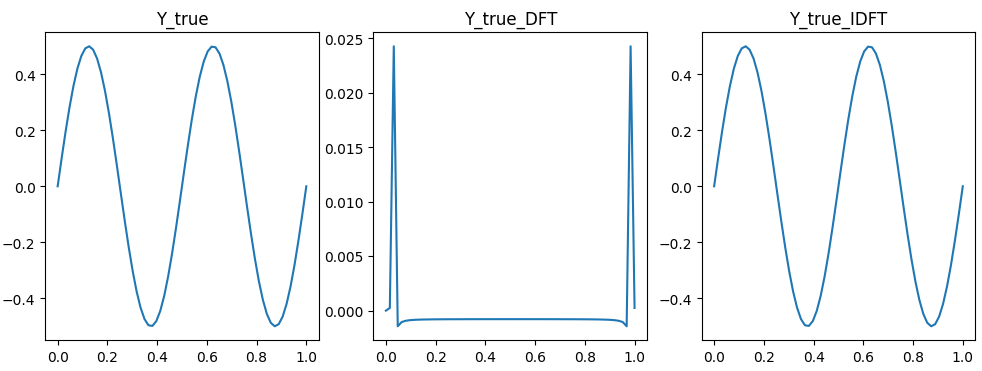
\includegraphics[width=0.6\linewidth]{fourier_1D_discret.png}
\end{minipage}

\paragraph{Transformée de Fourier continue \\}

\noindent La Transformée de Fourier continue (en 1D) est définie par :
$$F(u)=\int_{0}^{L}f(x)e^{-2i\pi ux}dx$$
L'inverse de la Transformée de Fourier continue (en 1D) est définie par :
$$f(x)=\int_{0}^{L}F(u)e^{2i\pi ux}du$$

Par la méthode des rectangles, on a :
$$F(u)\approx\frac{L}{N}\sum_{k=0}^{N-2}f(x_k)e^{-2i\pi ux_k} \quad \text{et} \quad f(x)\approx\frac{L}{N}\sum_{k=0}^{N-2}F(u_k)e^{2i\pi u_kx}$$

Voici l'implémentation Python de la transformée de Fourier continue et de son inverse :

\begin{lstlisting}
# Fourier Transform
def DFT(f,XX):
	N = f.shape[0]
	F = np.zeros(N,dtype=complex)
	for (k,u) in enumerate(XX):
		for (l,x) in enumerate(XX[:-1]):
			F[k]+=f[l]*cmath.exp(-2j*np.pi*x*u)
	return 1/N*F
\end{lstlisting}
\begin{lstlisting}
# Inverse Fourier Transform
def IDFT(F,XX):
	N = F.shape[0]
	f = np.zeros(N,dtype=complex)
	for (k,x) in enumerate(XX):
		for (l,u) in enumerate(XX[:-1]):
			f[k]+=F[l]*cmath.exp(2j*np.pi*u*x)
	return 1/N*f
\end{lstlisting}

\underline{Résultats :}

En prenant le même cas test que pour la transformée de Fourier discrète, voici les résultats obtenus :

\begin{minipage}{\linewidth}
	\centering
	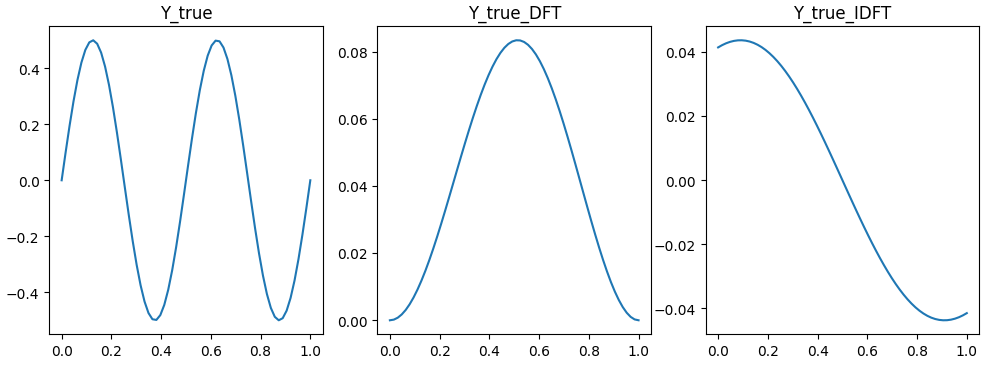
\includegraphics[width=0.6\linewidth]{fourier_1D_continu.png}
\end{minipage}

\begin{Rem}
	Il semblerait que la discrétisation du problème ne fonctionne pas. En effet dans la preuve que $f$ est bien la fonction réciproque de $F$ faite au-dessus (pour le cas discret), lorsque $x\ne x'$, on obtenait une série géométrique en faisant passer en exposant $u$. Dans notre cas, lorsque $x_k\ne x$, on ne peut pas mettre en exposant u, ce n'est pas un entier. Il faudrait trouver une solution à ce problème !
\end{Rem}

\subsubsection{Transformée de Fourier en 2D}

\paragraph{Transformée de Fourier discrète \\}

\noindent La Transformée de Fourier discrète (en 2D) est définie par :
$$F(u,v)=\frac{1}{N^2}\sum_{x=0}^{N-1}\sum_{y=0}^{N-1}f(x,y)e^{-i\frac{2\pi}{N}(ux+vy)}$$
L'inverse de la Transformée de Fourier discrète (en 2D) est définie par :
$$f(x,y)=\sum_{u=0}^{N-1}\sum_{v=0}^{N-1}F(u,v)e^{i\frac{2\pi}{N}(ux+vy)}$$

Voici l'implémentation Python de la transformée de Fourier discrète et de son inverse :

\lstset{style=Python}

\begin{lstlisting}
# Discrete Fourier Transform
def DFT(img):
	N = img.shape[0]
	img_DFT = np.zeros([N,N],dtype=complex)
	for u in range(N):
		for v in range(N):
			for x in range(N):
				for y in range(N):
					img_DFT[u,v]+=img[x,y]*cmath.exp(-2j*np.pi/N*(u*x+v*y))
	return 1/N**2*img_DFT
\end{lstlisting}
\begin{lstlisting}
# Inverse Discrete Fourier Transform
def IDFT(img_DFT): # Inverse Discrete Fourier Transform
	N = img_DFT.shape[0]
	img = np.zeros([N,N],dtype=complex)
	for x in range(N):
		for y in range(N):
			for u in range(N):
				for v in range(N):
					img[x,y]+=img_DFT[u,v]*cmath.exp(2j*np.pi/N*(u*x+v*y))
	return img
\end{lstlisting}

\underline{Résultats :}

On prendra
$$u_{ex}(x,y)=S\sin(2\pi fx + p)\sin(2\pi fy + p)$$
avec $S=0.5$ ,$f=2$ et $p=0$.

On peut y appliquer la DFT puis reconstruire l'image originale en y appliquant la DFT inverse. 

Voici les résultats obtenus avec nb\_vert=64 et $x,y\in[0,1]$ :

\begin{minipage}{\linewidth}
	\centering
	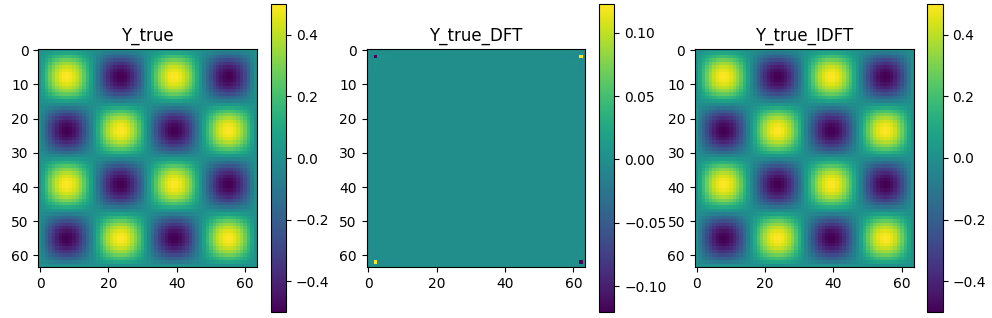
\includegraphics[width=0.6\linewidth]{fourier_2D_discret.png}
\end{minipage}

\paragraph{Transformée de Fourier continue \\}

Même problème que dans le cas 1D. A régler !

\subsection{Polynômes de Legendre}

\subsubsection{Polynômes de Legendre en 1D}

On cherche à décomposer une fonction en une série de polynômes de Legendre de la manière suivante :
\begin{equation}
	f(x)=\sum_{n=0}^{N-1} \alpha_n P_n(x)
	\label{decomp_1D}
\end{equation}
où les polynômes de Legendre sont définis pour tout $x\in\mathbb{R}$ par
$$P_n(x)=\frac{1}{2^n n!}\frac{d^n}{dx^n}[(x^2-1)^n]$$
On notera que les polynômes de Legendre sont orthogonaux dans l'espace $L^2(]-1,1[)$ et plus précisément
\begin{equation}
	\int_{-1}^1 P_n(x)P_m(x)dx=\frac{2}{2n+1}\delta_{nm} 
	\label{ortho_1D}
\end{equation}
On pose $X=(x_0,\dots,x_{N-1})$.

Ainsi
$$f(x_i)=\sum_{p=0}^{P-1}\alpha_p P_p(x_i), \quad \forall i\in\{0,\dots,N-1\}$$

On pose
$$\widetilde{F_N}=\begin{pmatrix}
	f(x_0) \\
	\vdots \\
	f(x_{N-1})
\end{pmatrix}\in\mathbb{R}^N, \quad \widetilde{\alpha_P}=\begin{pmatrix}
	\alpha_0 \\
	\vdots \\
	\alpha_{P-1}
\end{pmatrix}\in\mathbb{R}^P, \quad \widetilde{P_N}=\begin{pmatrix}
	P_0(x_0) & \dots & P_{P-1}(x_0) \\
	\vdots & \ddots & \vdots \\
	P_0(x_{N-1}) & \dots & P_{P-1}(x_{N-1})
\end{pmatrix}\in\mathcal{M}_{N,P}(\mathbb{R})$$

Par la méthode des rectangles (à gauche), \ref{ortho_1D} devient
\begin{align*}
	\int_{-1}^1 P_n(x)P_m(x)dx&=\sum_{i=0}^{N-2}\int_{x_i}^{x_{i+1}}P_n(x)P_m(x)dx \\
	&\approx \sum_{i=0}^{N-2} (x_{i+1}-x_i)P_n(x_i)P_m(x_i) \\
	&=\frac{2}{N}\sum_{i=0}^{N-2} P_n(x_i)P_m(x_i) \approx\frac{2}{2n+1}\delta_{nm} 
\end{align*}

On en déduit \color{red}PB 1\color{black}
\begin{equation}
	\frac{2}{N}\widetilde{P_N}^T\widetilde{P_N}=\widetilde{D_P}\label{diag_1D}
\end{equation}
avec
$$\widetilde{D_P}=diag\left(\frac{2}{2p+1},p=0,\dots,P-1\right)\in\mathcal{M}_P(\mathbb{R})$$

On cherche à déterminer $\widetilde{\alpha_P}$. Pour cela, on va réécrire le problème \ref{decomp_1D} sous la forme matricielle suivante
\begin{align*}
	\widetilde{P_N}\widetilde{\alpha_P}=\widetilde{F_N}& \\
	\iff \quad \widetilde{P_N}^T\widetilde{P_N}\widetilde{\alpha_P}=\widetilde{P_N}^T\widetilde{F_N}& \\
	\iff \quad \frac{N}{2}\widetilde{D_P}\widetilde{\alpha_P}=\widetilde{P_N}^T\widetilde{F_N}& \\
	\iff \quad \boxed{\widetilde{\alpha_P}=\frac{2}{N}\widetilde{D_P}^{-1}\widetilde{P_N}^T\widetilde{F_N}}&
\end{align*}
avec
$$\widetilde{D_P}^{-1}=diag\left(\frac{2p+1}{2},p=0,\dots,P-1\right)\in\mathcal{M}_P(\mathbb{R})$$

Autrement dit
$$\forall p\in\{0,\dots,P-1\}, \; \alpha_p = \frac{2p+1}{2}<f(X),P_p(X)>_{L^2(]-1,1[)}$$

\underline{Résultats :}

On prendra
$$u(x)=exp\left(-\frac{(x-\mu)^2}{2\sigma^2}\right)$$
avec $\mu=0$ et $\sigma=1$.

On prendra $P=10$ et $N=100$ et $x\in[-1,1]$.

On commence par vérifier l'orthogonalité des polynômes de Legendre :

\begin{minipage}{\linewidth}
	\centering
	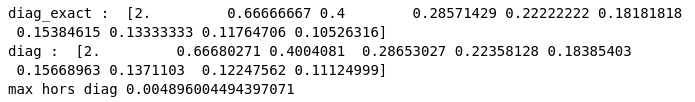
\includegraphics[width=0.6\linewidth]{legendre_1D_ortho.png}
\end{minipage}

\begin{Rem}
	A noter que pour calculer le produit scalaire sur $L^2(]-1,1[)$, on utilisera la méthode des trapèzes.
\end{Rem}

Voici les résultats obtenus pour la reconstruction de la fonction en utilisant la décomposition en une série de polynômes de Legendre :

\begin{minipage}{\linewidth}
	\centering
	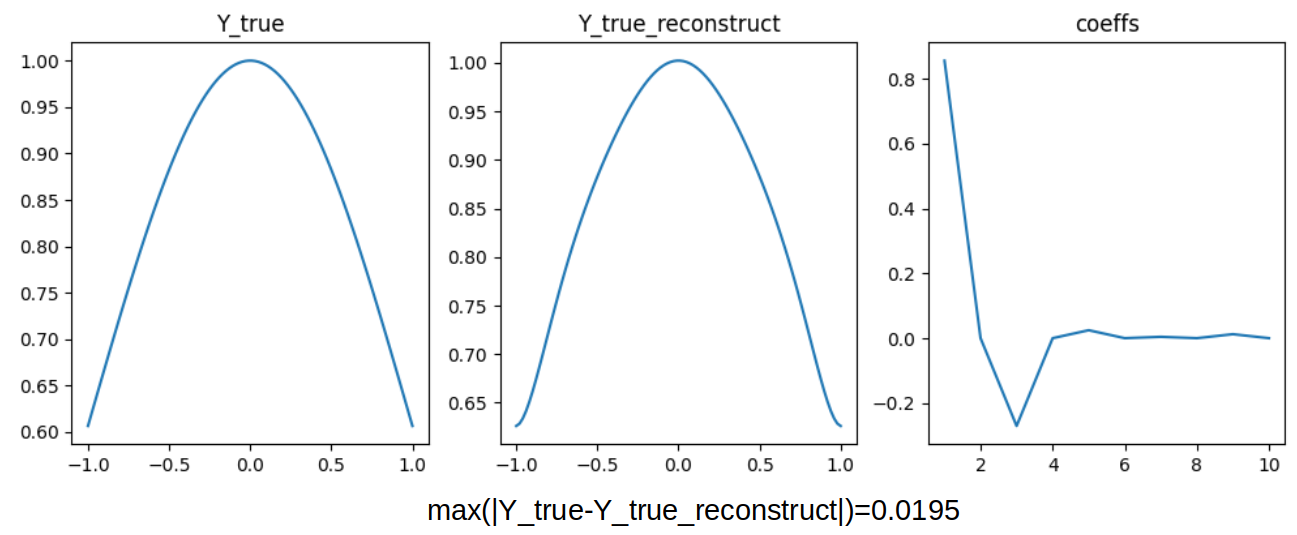
\includegraphics[width=0.5\linewidth]{legendre_1D_same.png}
\end{minipage}

On peut également reconstruire la fonction avec plus de points $N_2=1000$ :

\begin{minipage}{\linewidth}
	\centering
	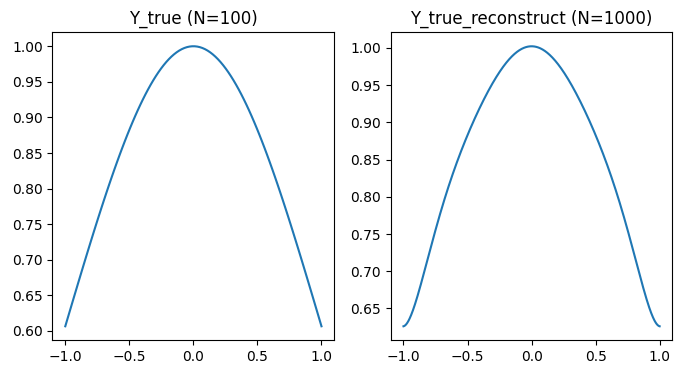
\includegraphics[width=0.4\linewidth]{legendre_1D_diff.png}
\end{minipage}

En faisant varier $N$ et $P$, on remarque que l'approximation semble dépendre énormément de $P$ :

\begin{minipage}{\linewidth}
	\centering
	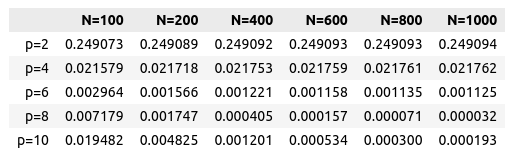
\includegraphics[width=0.4\linewidth]{legendre_1D_Np.png}
\end{minipage}

\subsubsection{Polynômes de Legendre en 2D}

On cherche à décomposer une fonction en une série de polynômes de Legendre de la manière suivante :
\begin{equation}
	f(x,y)=\sum_{p=0}^{P-1}\sum_{q=0}^{Q-1}\alpha_{p,q}P_p(x)P_q(y)
	\label{decomp}
\end{equation}
où les polynômes de Legendre sont définis pour tout $x\in\mathbb{R}$ par
$$P_n(x)=\frac{1}{2^n n!}\frac{d^n}{dx^n}[(x^2-1)^n]$$
On notera que les polynômes de Legendre sont orthogonaux dans l'espace $L^2(]-1,1[)$ et plus précisément
\begin{equation}
	\int_{-1}^1 P_n(x)P_m(x)dx=\frac{2}{2n+1}\delta_{nm} 
	\label{ortho}
\end{equation}
On pose $X=(x_0,\dots,x_{N-1})$ et $Y=(y_0,\dots,y_{M-1})$.

Ainsi
$$f(x_i,y_j)=\sum_{p=0}^{P-1}\sum_{q=0}^{Q-1}\alpha_{p,q}P_p(x_i)P_q(y_j), \quad \forall i\in\{0,\dots,N-1\},j\in\{0,\dots,M-1\}$$

On pose
$$\widetilde{F_{N,M}}=\begin{pmatrix}
	f(x_0,y_0) & \dots & f(x_0,y_{M-1}) \\
	\vdots & \ddots & \vdots \\
	f(x_{N-1},y_0) & \dots & f(x_{N-1},y_{M-1})
\end{pmatrix}\in\mathcal{M}_{N,M}(\mathbb{R})$$

$$\widetilde{\alpha_{P,Q}}=\begin{pmatrix}
	\alpha_{0,0} & \dots & \alpha_{0,Q-1} \\
	\vdots & \ddots & \vdots \\
	\alpha_{P-1,0} & \dots & \alpha_{P-1,Q-1}
\end{pmatrix}\in\mathcal{M}_{P,Q}(\mathbb{R})$$

$$\widetilde{P_N}=\begin{pmatrix}
	P_0(x_0) & \dots & P_{P-1}(x_0) \\
	\vdots & \ddots & \vdots \\
	P_0(x_{N-1}) & \dots & P_{P-1}(x_{N-1})
\end{pmatrix}\in\mathcal{M}_{N,P}(\mathbb{R})$$

$$\widetilde{P_M}=\begin{pmatrix}
	P_0(y_0) & \dots & P_{Q-1}(y_0) \\
	\vdots & \ddots & \vdots \\
	P_0(y_{M-1}) & \dots & P_{Q-1}(y_{M-1})
\end{pmatrix}\in\mathcal{M}_{M,Q}(\mathbb{R})$$

Par la méthode des rectangles (à gauche), \ref{ortho} devient
\begin{align*}
	\int_{-1}^1 P_n(x)P_m(x)dx&=\sum_{i=0}^{N-2}\int_{x_i}^{x_{i+1}}P_n(x)P_m(x)dx \\
	&\approx \sum_{i=0}^{N-2} (x_{i+1}-x_i)P_n(x_i)P_m(x_i) \\
	&=\frac{2}{N}\sum_{i=0}^{N-2} P_n(x_i)P_m(x_i) \approx\frac{2}{2n+1}\delta_{nm} 
\end{align*}

On en déduit \color{red}PB 1\color{black}
\begin{equation}
	\frac{2}{N}\widetilde{P_N}^T\widetilde{P_N}=\widetilde{D_P} \quad \text{et} \quad \frac{2}{M}\widetilde{P_M}^T\widetilde{P_M}=\widetilde{D_Q}
	\label{diag}
\end{equation}
avec
$$\widetilde{D_P}=diag\left(\frac{2}{2p+1},p=0,\dots,P-1\right)\in\mathcal{M}_P(\mathbb{R}) \quad \text{et} \quad \widetilde{D_Q}=diag\left(\frac{2}{2q+1},q=0,\dots,Q-1\right)\in\mathcal{M}_Q(\mathbb{R})$$

On cherche à déterminer $\widetilde{\alpha_{P,Q}}$. Pour cela, on va réécrire le problème \ref{decomp} sous la forme matricielle suivante
\begin{align*}
	\widetilde{P_N}\widetilde{\alpha_{P,Q}}\widetilde{P_M}^T=\widetilde{F_{N,M}}& \\
	\iff \quad \widetilde{P_N}^T\widetilde{P_N}\widetilde{\alpha_{P,Q}}\widetilde{P_M}^T\widetilde{P_M}=\widetilde{P_N}^T\widetilde{F_{N,M}}\widetilde{P_M}& \\
	\iff \quad \frac{NM}{4}\widetilde{D_P}\widetilde{\alpha_{P,Q}}\widetilde{D_Q}=\widetilde{P_N}^T\widetilde{F_{N,M}}\widetilde{P_M}& \\
	\iff \quad \boxed{\widetilde{\alpha_{P,Q}}=\frac{4}{NM}\widetilde{D_P}^{-1}\widetilde{P_N}^T\widetilde{F_{N,M}}\widetilde{P_M}\widetilde{D_Q}^{-1}}& \\
\end{align*}
avec
$$\widetilde{D_P}^{-1}=diag\left(\frac{2p+1}{2},p=0,\dots,P-1\right)\in\mathcal{M}_P(\mathbb{R}) \quad \text{et} \quad \widetilde{D_Q}^{-1}=diag\left(\frac{2q+1}{2},q=0,\dots,Q-1\right)\in\mathcal{M}_Q(\mathbb{R})$$

\color{red}
\textbf{Problèmes :}
\begin{enumerate}
	\item $\widetilde{P_N}^T\widetilde{P_N}$ fait un cran de trop ! On a un rectangle supplémentaire !
	\item Choisir $P$ et $Q$ : si on les prend trop grand, résultats incohérents !!!
\end{enumerate}
\color{black}

\begin{Rem}
	Pour $x\in[a,b]$, on fait un changement de variable pour se ramener dans l'intervalle $[-1,1]$. \\
	On pose alors
	$$\tilde{x}=\frac{2}{b-a}x+\frac{a+b}{a-b}$$
	Ainsi
	$$\tilde{f}(\tilde{x})=f(x)$$
\end{Rem}


\underline{Résultats :}

On prendra
$$u(x)=exp\left(-\frac{(x-\mu)^2+(y-\mu)^2}{2\sigma^2}\right)$$
avec $\mu=0$ et $\sigma=1$.

On prendra $P,Q=5$ et $N=100$ et $x\in[-1,1]$.

On commence par vérifier l'orthogonalité des polynômes de Legendre :

\begin{minipage}{\linewidth}
	\centering
	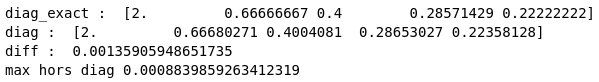
\includegraphics[width=0.6\linewidth]{legendre_2D_ortho.png}
\end{minipage}

\begin{Rem}
	A noter que contrairement au cas 1D, pour calculer le produit scalaire sur $L^2(]-1,1[)$, on utilise cette fois le produit matricielle $\frac{2}{N}P_NP_N^T$. Il faut améliorer ceci !
\end{Rem}

Voici les résultats obtenus pour la reconstruction de l'image en utilisant la décomposition en une série de polynômes de Legendre :

\begin{minipage}{\linewidth}
	\centering
	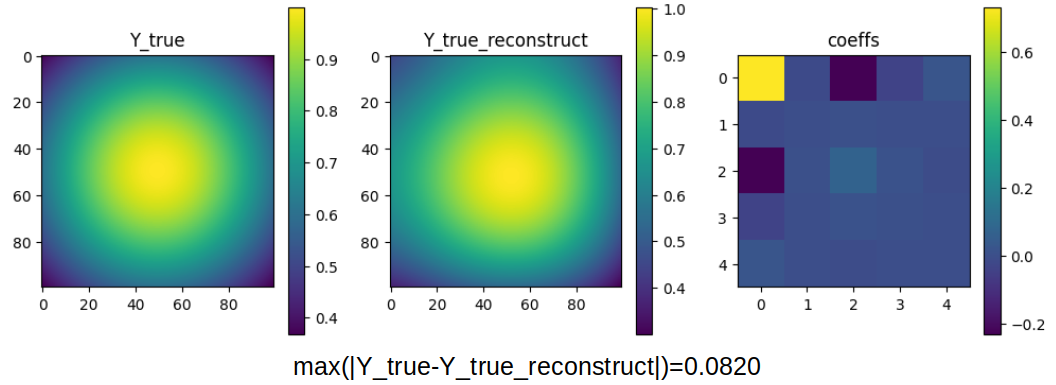
\includegraphics[width=0.7\linewidth]{legendre_2D_same.png}
\end{minipage}

\newpage

On peut également reconstruire la fonction avec plus de points $N_2=500$ :

\begin{minipage}{\linewidth}
	\centering
	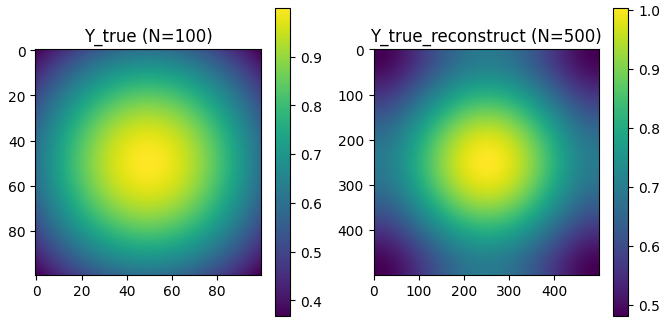
\includegraphics[width=0.5\linewidth]{legendre_2D_diff.png}
\end{minipage}

En faisant varier $N$ et $P$, on remarque que l'approximation semble dépendre énormément de $P$ :

\begin{minipage}{\linewidth}
	\centering
	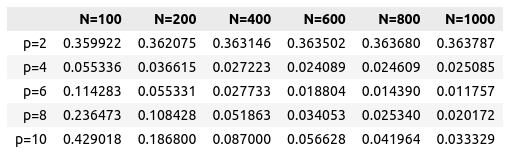
\includegraphics[width=0.4\linewidth]{legendre_2D_Np.png}
\end{minipage}

\begin{Rem}
	Problème au niveau du produit scalaire !
\end{Rem}

\subsection{Test sur le FNO}

\subsubsection{Explication}

On considère $\Omega$ le cercle de rayon $\sqrt{2}/4$ et de centre $(0.5,0.5)$ avec $\Phi(x,y)=1/8-(x-1/2)^2-(y-1/2)^2$ et le domain fictif $O=(0,1)^2$.

On souhaite résoudre 
\begin{equation*}
	\begin{cases}
		-\Delta u &= f\,, \quad \text{dans $\Omega$}\,, \\
		u &= 0\,, \quad \text{sur $\Gamma$}\,, \\
	\end{cases}
\end{equation*}
où 
$$f(x,y) = \exp\left(-\frac{(x-\mu_0)^2 + (y-\mu_1)^2}{2\sigma^2}\right)\,, $$ 
avec $\sigma \sim \mathcal{U}([0.1,0.6])$ et $\mu_0, \mu_1 \sim \mathcal{U}([0.5-\sqrt{2}/4, 0.5+\sqrt{2}/4])$.

On cherche à tester et comparer 2 méthodes de correction sur le FNO :

\begin{enumerate}[label=\textbullet]
	
	\item \textbf{Méthode 1 :}
	
	\textbf{Sans rehaussement :}
	
	On souhaite résoudre le problème suivant
	$$\left\{\begin{aligned}
		&-\Delta (\tilde{\phi}C)=f \quad &&\Omega \\
		&\tilde{\phi}C=0 \quad &&\Gamma
	\end{aligned}\right.$$
	On pose $\tilde{u}=\tilde{\phi}C$.
	On utilise alors la formulation $\Phi$-FEM classique (en homogène).
	
	\textbf{Avec rehaussement :}
	
	On souhaite résoudre le problème suivant
	$$\left\{\begin{aligned}
		&-\Delta (\hat{\phi}C)=f \quad &&\Omega \\
		&\hat{\phi}C=m \quad &&\Gamma
	\end{aligned}\right.$$
	On pose $\hat{u}=\hat{\phi}C$.
	On utilise alors la formulation $\Phi$-FEM en imposant la condition au bord par la méthode duale.
	
	\item \textbf{Méthode 2 :}
	
	On souhaite résoudre le problème suivant
	$$\left\{\begin{aligned}
		&-\Delta(\phi C)=\tilde{f} \quad &&\Omega \\
		&\tilde{C}=0 \quad &&\Gamma
	\end{aligned}\right.$$
	avec $\tilde{u}=\tilde{\phi}+\tilde{C}$ où $\tilde{C}=\phi C$ et $\tilde{f}=f+\Delta\tilde{\phi}$.
	On utilise alors la formulation $\Phi$-FEM classique (en homogène).
	
\end{enumerate}

\subsubsection{Applications}

Voici les étapes effectuées :

\begin{enumerate}[label=\textbullet]
	\item On va créer une classe prenant en paramètre nb\_vert. On récupère alors \textit{nb\_dofs}=2\textit{nb\_vert}-1.
	\item On récupère les paramètres \textit{params} de l'ancien échantillon test ainsi que le nombre de données \textit{nb\_data}.
	\item On crée nos nouveaux inputs \textit{X\_test} pour l'échantillon test de taille (\textit{nb\_data},\textit{nb\_dofs},\textit{nb\_dofs},\textit{nb\_channels}).
	\item On génère nos \textit{nb\_data} solution sur-raffinées \textit{Y\_test} avec FEniCS.
	\item On sépare notre échantillon test en batch pour éviter les Out Of Memory. Ainsi, pour chaque batch, on récupère la prédiction du FNO \textit{Y\_pred} et les erreurs associées \textit{errors\_FNO} (par rapport aux solutions sur-raffinées).
	\item On calcule $\widetilde{P_N}$ et $\widetilde{P_M}$ puis $\widetilde{\alpha_{P,Q}}$.
	\item On reconstruit alors les solutions en utilisant les polynômes de Legendre.
	\item On calcule ensuite les deux erreurs suivantes :
	\begin{itemize}
		\item max(|Y\_pred-Y\_pred\_reconstruct|) -> errors\_legendre
		\item $||Y\_test-\phi Y\_pred\_reconstruct||_{L^2}$  -> errors\_reconstruct
	\end{itemize}
\end{enumerate}

\begin{Rem}
	On notera que les Y\_pred sont $w$ (et non $u$), il manque la multiplication par $\phi$.
\end{Rem}

Voici les errors\_legendre obtenues sans le masque en fonction des époques :

\begin{minipage}{\linewidth}
	\centering
	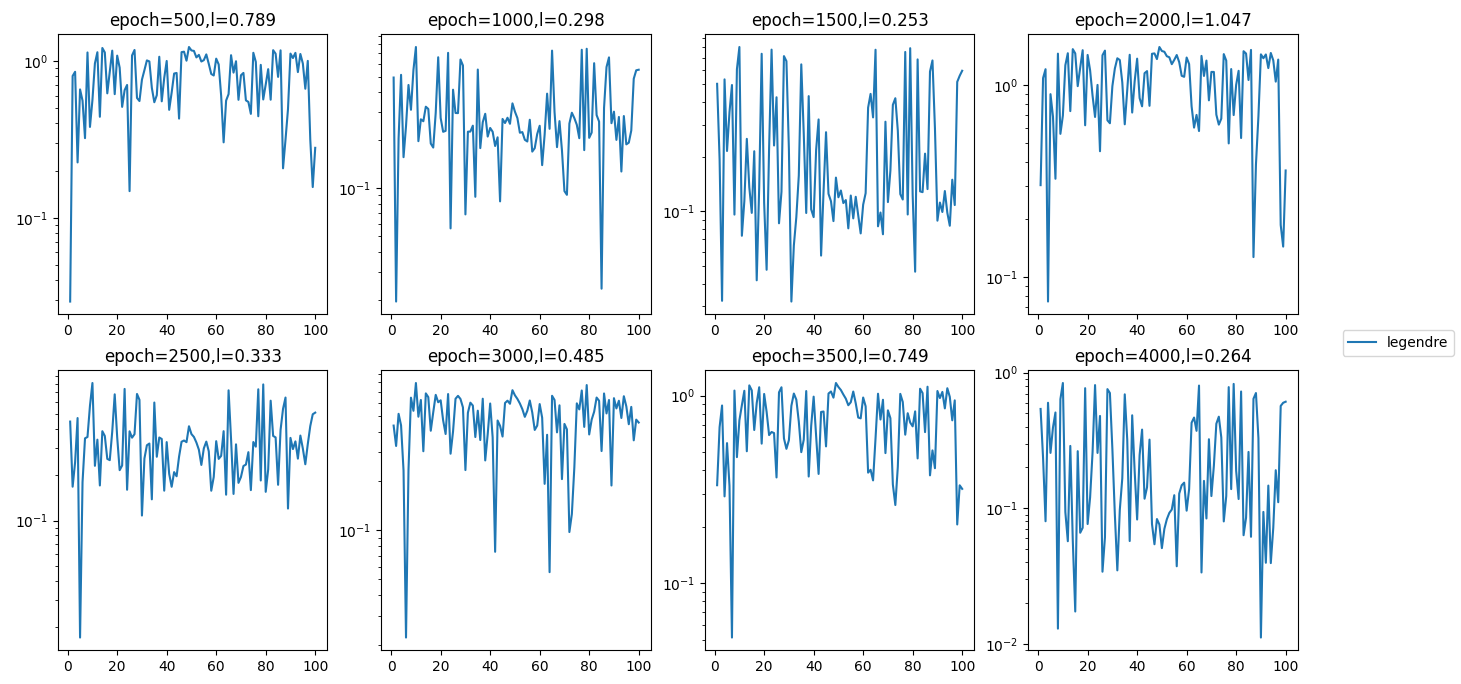
\includegraphics[width=0.9\linewidth]{FNO_errors_legendre_without_mask.png}
\end{minipage}

Et voici deux cas tests sans le masque (epoch=500, data=0,1)):

\begin{minipage}{\linewidth}
	\centering
	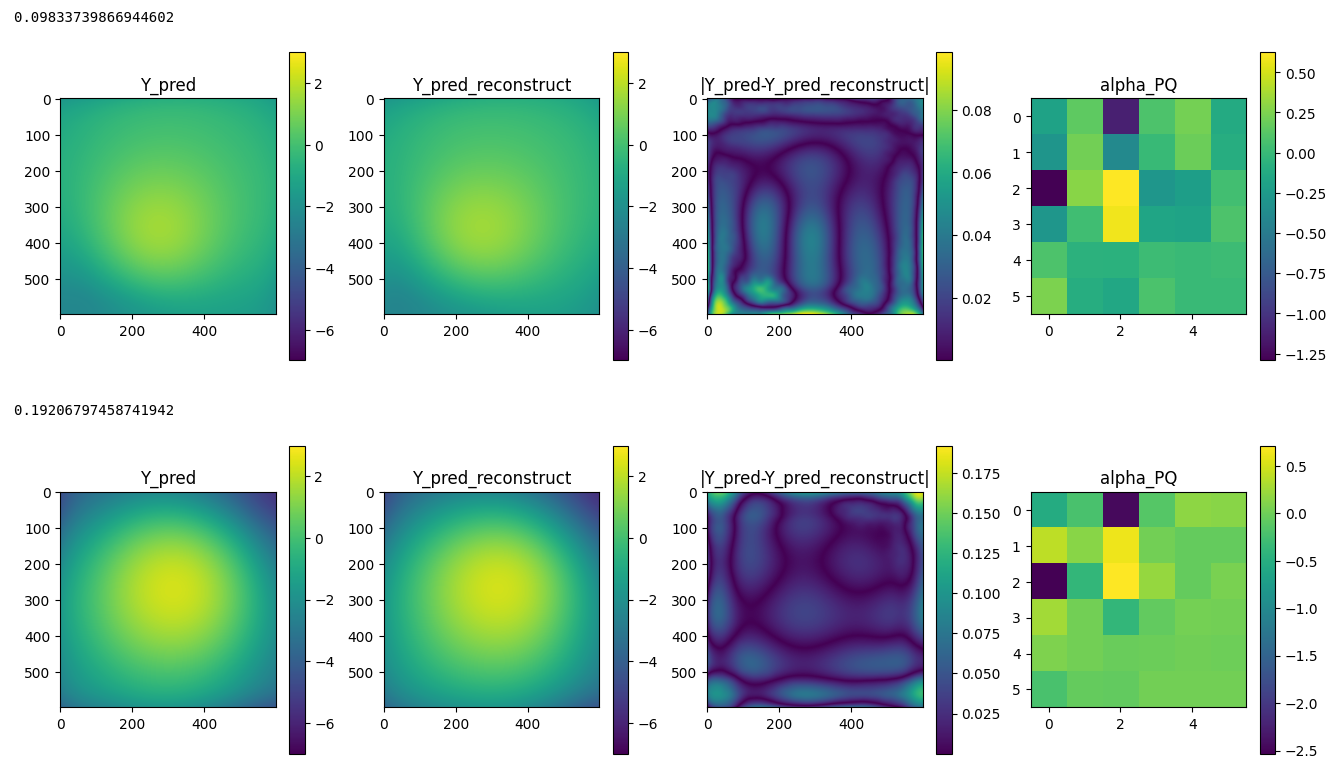
\includegraphics[width=0.7\linewidth]{FNO_test_cases_without_mask.png}
\end{minipage}

Après avoir visualisé les cas test, il semblerait que les grosses erreurs se fassent aux bords, ce qui ne devrait pas posé problème étant donné que l'on va appliquer un masque.

\newpage

Voici les 2 mêmes cas tests avec le masque :

\begin{minipage}{\linewidth}
	\centering
	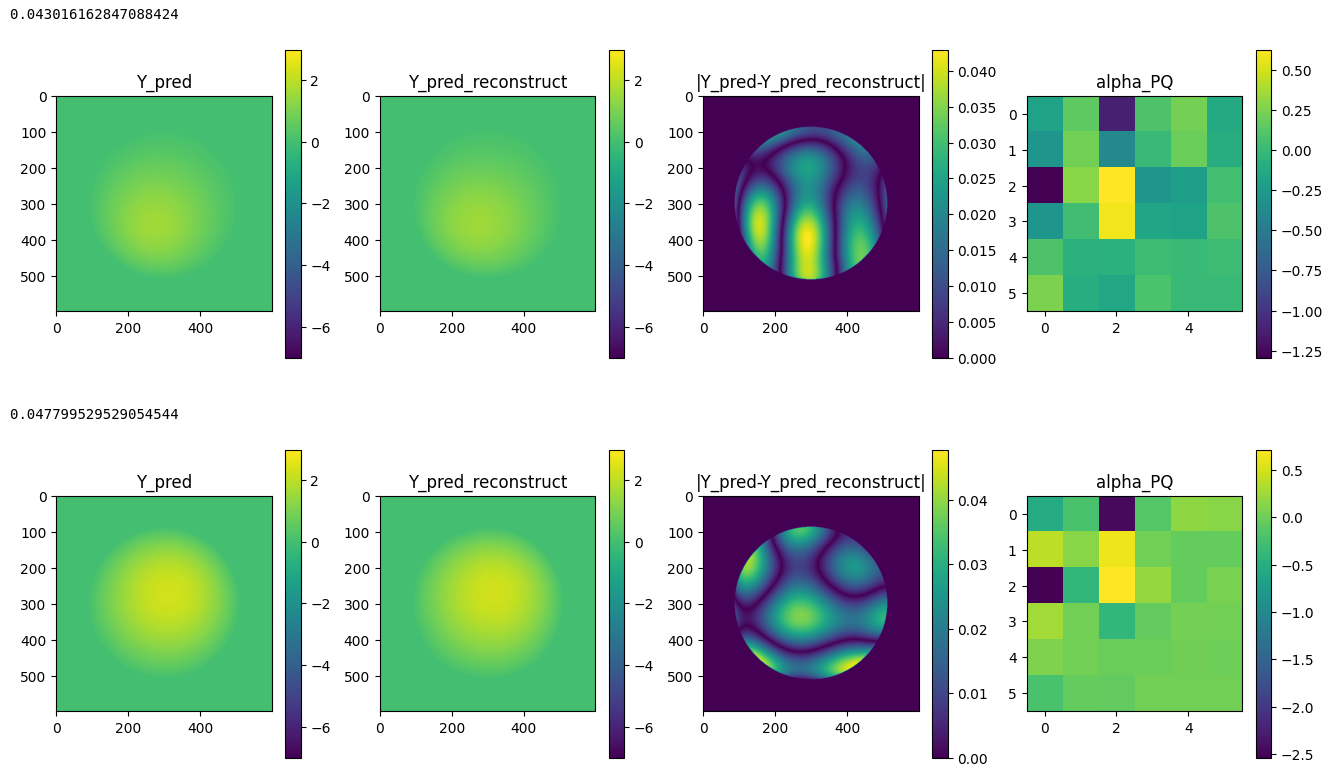
\includegraphics[width=0.7\linewidth]{FNO_test_cases_with_mask.png}
\end{minipage}

En multipliant Y\_pred\_reconstruct par $\phi$, on peut alors obtenir les erreurs comparés à la solution sur-raffinée :

\begin{minipage}{\linewidth}
	\centering
	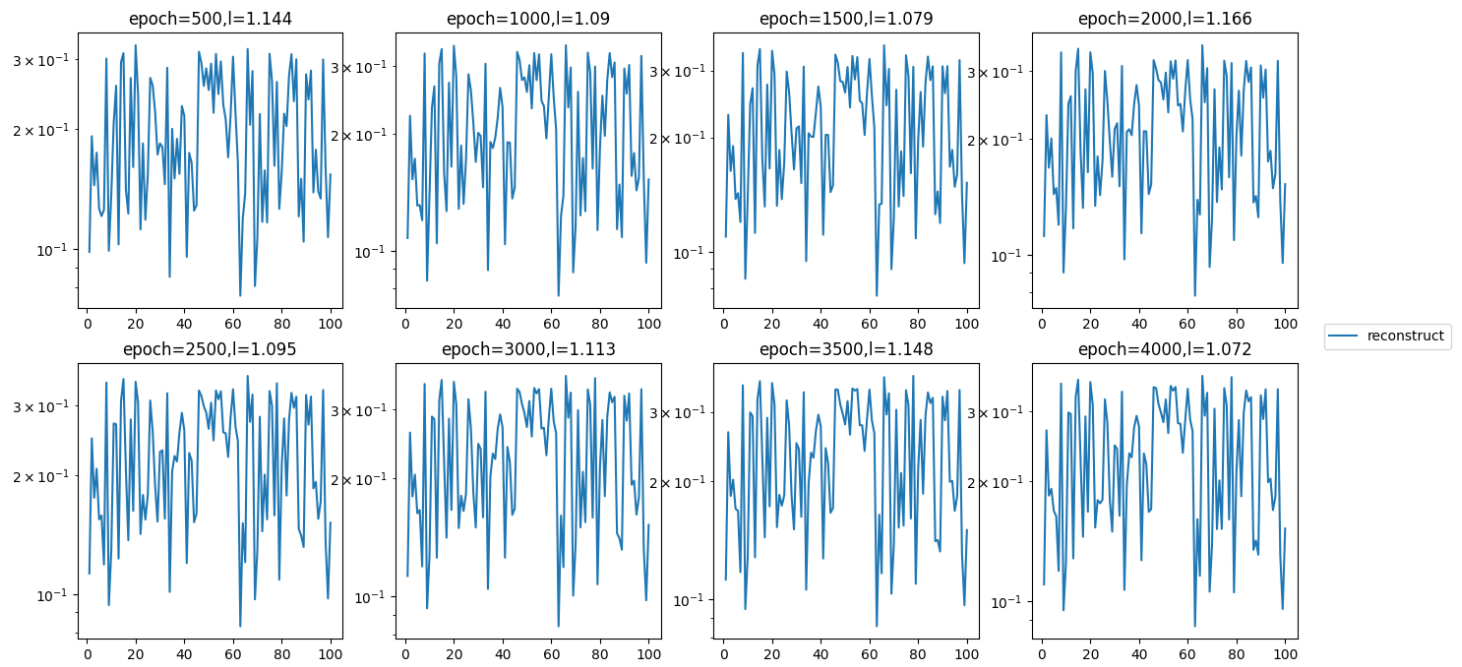
\includegraphics[width=0.7\linewidth]{FNO_errors_reconstruct_with_mask.png}
\end{minipage}

\conclusion{Il semblerait que les polynômes de Legendre permettent bien d'obtenir une solution analytique à partir de la solution produite par le FNO. La semaine prochaine, il faudra tester la correction en $\mathbb{P}^10$. On pourra également tester de décomposer directement $\phi\times$Y\_pred en série de polynômes de Legendre}
